\chapter{Simulation results} \label{ch:results}
In this section the results from training the controller algorithm in simulation will be presented. This is done by first introducing the fixed gain parameters in the PD algorithm and the initial parameters in the DDPG algorithm. This is followed by an implementation of two different \textit{reward function} designs, and the result from these. To conclude the chapter a discussion about the performance of the algorithm will be presented.\\\\
As discussed in chapter \ref{chap:method} the PD algorithm was initially tuned to make sure that the states ($\phi, \theta, z$) were stable on their own. This was done by giving the vehicle a fixed thrust in the $x$ direction, which resulted in the following proportional and derivative gains
\begin{align}
    K_{p} & = 1 \\
    K_{d} & = 0.1
\end{align}
In order to sufficiently train the DDPG algorithm the simulation was executed over $N = 400$ episodes, where each episode consisted of $t = [1, T=1000]$ steps. For each episode the algorithm will therefore be executed until T = 1000 \textbf{or} the BlueROV2 reaches the terminal state, indicating that it has reached the desired pose. The reward discount factor ($\gamma$), learning rate for the actor network ($\alpha_{a}$), learning rate for the critic network ($\alpha_{q}$) and the exploitation/exploration factor ($\epsilon$) were initially defined as
\begin{align}
    \gamma & = 0.9 \\
    \alpha_{a} & = 1e-4 \\
    \alpha_{q} & = 1e-4 \\
    \epsilon & = 1
\end{align}
Recall that $\alpha_{a}, \alpha_{q}$ and $\epsilon$ should all decrease over the number of iteration, since the algorithm gains larger and larger knowledge about the environment. This was by discounting the parameters at each episode, $N_{i}$ $(i = 1,...,400)$.\\\\
To accomplish Station Keeping the desired pose were defined as
\begin{align}
    s_{d} & = [x_{d}, y_{d}, \psi_{d}] = [1, 1, 0] \\
    s_{d,PD} & = [z_{d}, \phi_{d}, \theta_{d}] = [0, 0, 0]
\end{align}
Meaning that the BlueROV2 should stabilise at [$x = 1, y = 1$] in (NED). In order to evaluate performance of the algorithm there was created a vector containing information about the \textit{mean value} over the latest 100 total rewards, [$R_{N_{i-100}}, ..., R_{N_{i}}$], where $i = [1, 400]$. Hereafter, named the \textit{mean total reward vector}. The reason for doing this, especially taking the mean value, is because of uncertainties in the measurements. 
\section{Simulation 1}
\subsection*{Reward function}
As mentioned in chapter \ref{chap:method}, the reward function design is critical for the performance of the algorithm. Initially the reward function was defined with respect to the BlueROV2s' distance to the desired state, meaning that a larger distance should give a lower reward. The reward function, $r(s_{t}, a_{t})$, was therefore defined as

\begin{algorithm}[H]
\SetAlgoLined
\begin{align}
    r(s_{t}, a_{t}) & = \frac{1}{\norm{s_{e}}} \\
    s_{e} & = s_{d} - s_{t} \\
    R_{N_{i}} & += r(s_{t}, a_{t})
\end{align}
\caption{Reward function, Simulation 1}
\label{alg:reward_func_1}
\end{algorithm}
\subsection*{Simulation results 1}
By plotting the \textit{mean total reward vector} over all episodes, the result in figure \ref{fig:sim1} was obtained. 
\begin{figure}[H]
    \centering
    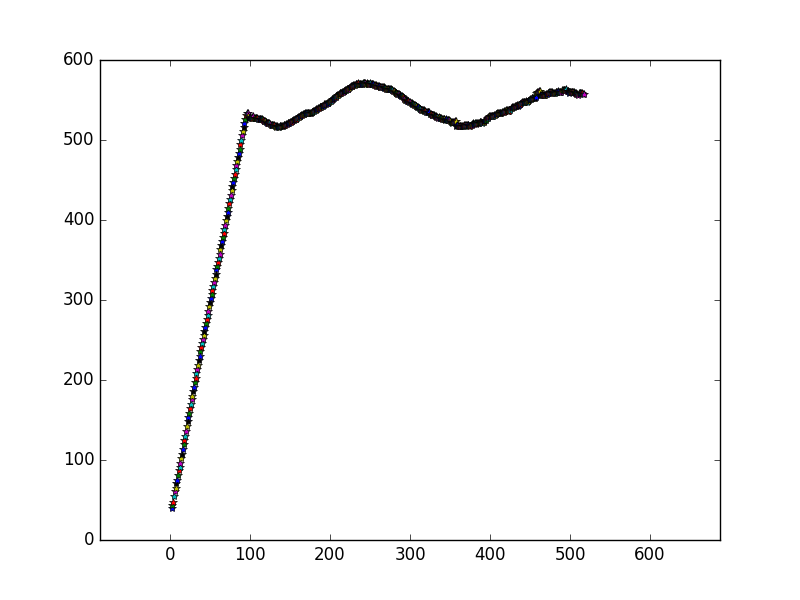
\includegraphics[width=0.7\textwidth]{images/chap5/figure_1.png}
    \caption{Simulation 1}
    \label{fig:sim1}
\end{figure}
In figure \ref{fig:sim1} the $y-axis$ specifies the total reward, and the $x-axis$ specifies number of episode. From the figure we see that the total reward converges to an oscillating value. Since the figure displays the mean value over the 100 latest episodes it is expected that the graph converges to a constant value, because the algorithm should learn the optimal action to take in every state, which results in the total reward being constant in each episode after it has learned the optimal behaviour. However, as previously stated the episodes is defined in such a way that the algorithm will be executed until T = 1000, or the BlueROV2 reaches the terminal state. This means that although it receives the highest reward at the desired position the episode will also terminate at this position, meaning that it will receive a larger total reward, $R_{N}$, by circulating the desired pose for $t=[1,T]$. This shows the importance of the reward function design, since the algorithm is able to find the optimal policy in each state, but the framework defined by the reward function is not optimal. 
\section{Simulation 2}
\subsection*{Reward function}
From the knowledge gained in simulation 1 it was clear that the reward function needed to be redesigned, in order to compensate for the fact that the algorithm received larger rewards for circulating the desired pose compared to reaching the terminal state. The new reward function was therefore defined as

\begin{algorithm}[H]
\SetAlgoLined
\begin{align}
    r(s_{t}, a_{t}) & = \frac{1}{\norm{s_{e}}} \\
    r(s_{t}, a_{t}) & += -0.05*t
\end{align}
    \If{abs($s_{e}$[0]) $<$ 0.1 \textbf{and} abs($s_{e}$[1]) $<$ 0.1}{
    r += 20 \\
    done = \textbf{True}
    }
    \If{$s_{e, diff}$[0] $<$ 0 \textbf{and} abs($s_{e, diff}$[1]) $<$ 0}{
    r += -5
    }
\caption{Reward function, Simulation 2}
\label{alg:reward_func_2}
\end{algorithm}
The algorithm now receives a negative reward, or a penalty, at each step $t$, meaning that it accomplishes the greatest total reward when reaching the desired pose using minimum steps. This will therefore prevent circulating the desired pose being the optimal behaviour. In algorithm \ref{alg:reward_func_2} there is also included two \textit{if}-sentences, where the first one checks the absolute error in the $x-$ and $y$ position. The reason for neglecting the error in $\psi$ here is that this state is valued less than the other two states. For Station Keeping the $x-$ and $y$ positions are more "\textit{relevant}". The second if-sentence evaluates $s_{e,diff}$, which is defined as the difference between the current error values and the error values in the previous step, $t-1$. If this difference is negative it means that the AUV moves away from the desired pose.
\subsection*{Simulation results 2}
By plotting the \textit{mean total reward vector} over all episodes, the result in figure \ref{fig:sim2} was obtained.
\begin{figure}[H]
    \centering
    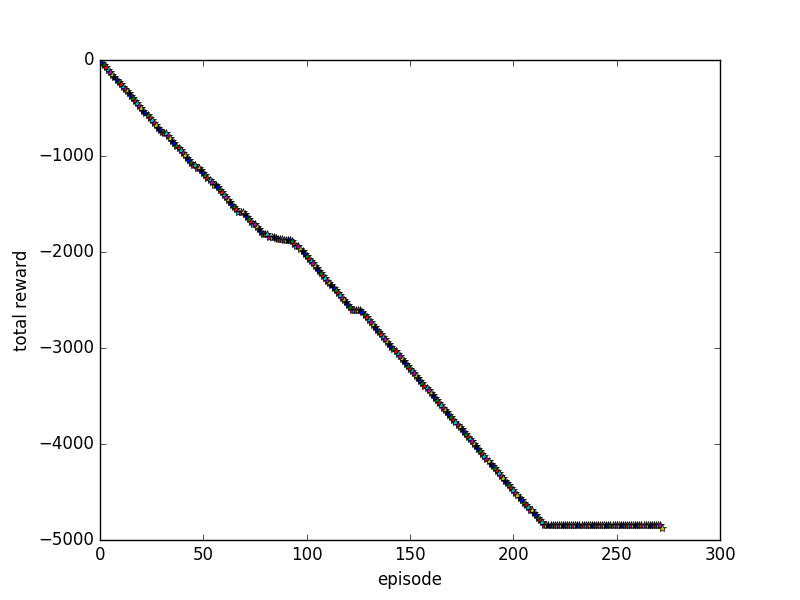
\includegraphics[width=0.7\textwidth]{images/chap5/figure_1-1.png}
    \caption{Simulation 2}
    \label{fig:sim2}
\end{figure}
The result from simulation 2 is illustrated in figure \ref{fig:sim2}. Here we see that the algorithm converges to a constant total reward of $\approx$ -4800 after $\approx$ 215 episodes. Compared to simulation 1 the oscillating behaviour is removed, and the agent moves straight to the desired pose in every episode. The algorithm has therefore \textit{successfully} converged to reach the desired pose for Station Keeping.

\section{Performance evaluation}
In order to evaluate the performance of the algorithm, an performance evaluation algorithm was constructed. This algorithm has the same form as the controller, the only difference being that it only uses the optimal policy learned during training, and do not explore any new actions. This means that in any state, $s_{t}$, the evaluation algorithm will look at the stored possible actions in that state, and choose the action that resulted in the highest total cumulative reward.\\\\
When evaluating the algorithm in simulation 2 at the desired pose, given by $s_{d}=[x_{d},y_{d},\psi_{z}]=[1,1,0]$, the vehicle moves straight to the desired pose. However, the problem occurs when the vehicle i trying to obtain Station Keeping at this pose. Recall from algorithm \ref{alg:RF} that when the vehicle reaches the desired pose, it has reached the \textit{terminal state}. From chapter \ref{chap: deep} it was shown that the terminal state was necessary to prove convergence of the algorithm, and that the state indicates that the episode is \textit{done}. Although, the algorithm has successfully learned how to reach the Station Keeping pose, it expects that the episode is finished, because this is what it should expect from training. This means that the algorithm has no clue of which actions to take after the desired pose is reached, although it should make sure that the vehicle stays in this pose.\\\\
This problem is not because of the capabilities of the algorithm itself, but the framework defined for it in programming. More specifically wrongful design of the reward function. In order to resolve this the reward function therefore needs to be re-designed once again. As stated earlier in the section, the terminal state can \textit{not} be removed, since this may result in the algorithm not being able to find the optimal solution. However, one way to resolve the problem could be to include a \textit{time} constraint in algorithm \ref{alg:reward_func_2}, to ensure that the terminal state is not reached until the vehicle has stayed in the desired pose for a specific time period. A second approach to resolve the issue could also be to increase the simulation time, as well as reducing the exploration versus exploitation rate, $\epsilon$, less frequently. This would allow the algorithm to explore new actions for several more simulations, and could result in accomplishment of Station Keeping without adding a time constraint. However, both these approaches will be left as an implementation for \textit{future work} on the topic, because of minimum time to implement them. 